\documentclass[11pt]{article}

\usepackage[letterpaper,margin=0.88in,headheight=22pt]{geometry}
\usepackage{fontspec}
\IfFontExistsTF{Charis SIL}{\setmainfont{Charis SIL}}{\setmainfont{TeX Gyre Pagella}}
\IfFontExistsTF{Arimo}{\setsansfont{Arimo}}{\setsansfont{TeX Gyre Heros}}
\usepackage{microtype}
\usepackage{amsmath,amssymb}
\usepackage{siunitx}
\usepackage{booktabs}
\usepackage{tabularx}
\usepackage{longtable}
\usepackage{array}
\usepackage{enumitem}
\usepackage{xcolor}
\usepackage{colortbl}
\usepackage{graphicx}
\usepackage{tikz}
\usetikzlibrary{arrows.meta,positioning,calc,decorations.pathreplacing}
\usepackage[most]{tcolorbox}
\usepackage{titlesec}
\usepackage{fancyhdr}
\usepackage{caption}
\usepackage{float}
\usepackage[hidelinks]{hyperref}
\usepackage{lastpage}
\usepackage{needspace}
\usepackage{graphbox} % Extends graphicx

% University of Texas at Austin brand palette
\definecolor{UTBurntOrange}{HTML}{BF5700}
\definecolor{UTCharcoal}{HTML}{333F48}
\definecolor{UTLightOrange}{HTML}{F8971F}
\definecolor{UTWarmGray}{HTML}{D6D2C4}
\definecolor{UTSlate}{HTML}{9CADB7}
\definecolor{UTBlue}{HTML}{005F86}
\definecolor{UTBlueBright}{HTML}{00A9B7}
\definecolor{UTWarmLight}{HTML}{F6F5F2}
\definecolor{UTBlueLight}{HTML}{EEF5F7}
\definecolor{UTGrayLight}{HTML}{F4F5F6}

% Backward-compatible semantic aliases used throughout the document
\colorlet{Navy}{UTCharcoal}
\colorlet{Teal}{UTBurntOrange}
\colorlet{LightTeal}{UTBlueLight}
\colorlet{LightBlue}{UTWarmLight}
\colorlet{LightGray}{UTGrayLight}
\colorlet{MidGray}{UTCharcoal!78}
\colorlet{RuleGray}{UTWarmGray}
\colorlet{Warn}{UTLightOrange}
\colorlet{LightWarn}{UTWarmLight}

\hypersetup{
  colorlinks=true,
  linkcolor=UTBurntOrange,
  urlcolor=UTBlue,
  citecolor=UTCharcoal,
  pdftitle={STNCL Phase-Specific Experimental Plan},
  pdfauthor={TRIDENT Collaboration (UT Austin, ACU, VCU)}
}

\sisetup{
  detect-all,
  per-mode=symbol,
  range-phrase=--,
  range-units=single,
  group-separator={,},
  group-minimum-digits=4,
  group-digits=integer
}

\setlength{\parindent}{0pt}
\setlength{\parskip}{5.5pt}
\setlength{\emergencystretch}{1.5em}
\setlist[itemize]{leftmargin=1.35em,itemsep=2.5pt,topsep=3pt}
\setlist[enumerate]{leftmargin=1.55em,itemsep=3pt,topsep=3pt}
\renewcommand{\arraystretch}{1.18}
\titlespacing{\paragraph}{0pt}{0.5ex plus 0.5ex minus .2ex}{1em}

\titleformat{\section}
  {\Large\sffamily\bfseries\color{UTBurntOrange}}
  {\thesection}{0.65em}{}
  [\vspace{1pt}\color{UTWarmGray}\titlerule]
\titleformat{\subsection}
  {\large\sffamily\bfseries\color{UTCharcoal}}
  {\thesubsection}{0.6em}{}
\titleformat{\subsubsection}
  {\normalsize\sffamily\bfseries\color{UTCharcoal}}
  {\thesubsubsection}{0.55em}{}
\titlespacing*{\section}{0pt}{14pt}{7pt}
\titlespacing*{\subsection}{0pt}{11pt}{4pt}
\titlespacing*{\subsubsection}{0pt}{8pt}{2pt}

% Keep a heading from being stranded alone at the bottom of a page:
% require room for the title plus a few body lines, else break to the next page.
\usepackage{etoolbox}
\pretocmd{\section}{\needspace{5\baselineskip}}{}{}
\pretocmd{\subsection}{\needspace{7\baselineskip}}{}{}
\pretocmd{\subsubsection}{\needspace{5\baselineskip}}{}{}

\pagestyle{fancy}
\fancyhf{}
\fancyhead[L]{\small\sffamily\color{UTCharcoal}Prop-30 Glycol STNCL \textbullet\ TRIDENT}
\fancyhead[R]{\small\sffamily\color{UTBurntOrange}\PhaseDocShort -- Draft}
\fancyfoot[L]{\small\sffamily\color{UTCharcoal!78}Revision 0.1}
\fancyfoot[R]{\small\sffamily\color{UTCharcoal!78}Page \thepage\ of \pageref{LastPage}}
\renewcommand{\headrulewidth}{0.65pt}
\renewcommand{\headrule}{\hbox to\headwidth{\color{UTBurntOrange}\leaders\hrule height \headrulewidth\hfill}}
\renewcommand{\footrulewidth}{0pt}

\newtcolorbox{recommendbox}[1][]{
  enhanced,
  breakable,
  colback=UTWarmLight,
  colframe=UTBurntOrange,
  colbacktitle=UTBurntOrange,
  boxrule=0.7pt,
  arc=1.2mm,
  left=3mm,right=3mm,top=2.4mm,bottom=2.4mm,
  title={#1},
  fonttitle=\sffamily\bfseries,
  coltitle=white
}

\newcommand{\Tavg}{T_{\mathrm{avg},4}}
\newcommand{\Tdiag}{T_{\mathrm{diag}}}
\newcommand{\Thot}{T_{\mathrm{hot}}}
\newcommand{\Tcold}{T_{\mathrm{cold}}}
\newcommand{\QHs}{\dot Q_{H}^{s}}
\newcommand{\QCs}{\dot Q_{C}^{s}}
\newcommand{\mdotp}{\dot m_{p}}
\newcommand{\mdotpH}{\dot m_{p,H}}
\newcommand{\mdotpC}{\dot m_{p,C}}
\newcommand{\Tamb}{T_{\mathrm{amb}}}
\newcommand{\Rey}{\mathrm{Re}}
\newcommand{\Realpart}[1]{\Re\left(#1\right)}

\newcommand{\PhaseDocShort}{Phase 0: System Checkout}

% Cross-document names used instead of duplicating material owned by another phase.
\newcommand{\PhaseZeroDoc}{\textit{Phase 0 --- System Checkout}}
\newcommand{\PhaseOneDoc}{\textit{Phase 1 --- Ambient-Equilibrium Baseline}}
\newcommand{\PhaseTwoDoc}{\textit{Phase 2 --- Thermal Relaxation Tests}}
\newcommand{\PhaseThreeDoc}{\textit{Phase 3 --- Low-Duty Steady Heat-Loss Tests}}
\newcommand{\PhaseFourDoc}{\textit{Phase 4 --- Initial Test Matrix and Transition Characterization}}

\begin{document}
\hypersetup{pageanchor=false}

\begin{titlepage}
\thispagestyle{empty}
\begin{tikzpicture}[remember picture,overlay]
  \fill[UTBurntOrange] (current page.north west) rectangle ([yshift=-0.16in]current page.north east);
  \fill[UTWarmLight] ([yshift=1.45in]current page.south west) rectangle (current page.south east);
  \fill[UTBurntOrange] (current page.south west) rectangle ([yshift=0.16in]current page.south east);
\end{tikzpicture}

\noindent
\includegraphics[width=2.5in]{images/TRIDENT_logo.png}

{\color{UTWarmGray}\rule{\textwidth}{0.8pt}}
\vspace{0.24in}
\begin{tcolorbox}[
  enhanced, frame hidden, colback=white, boxrule=0pt,
  borderline west={4pt}{0pt}{UTBurntOrange},
  left=5mm,right=0mm,top=1mm,bottom=1mm, sharp corners
]
{\raggedright\sffamily\bfseries\fontsize{23}{27}\selectfont\color{UTCharcoal}
Experimental Plan for the Initial Characterization of the Prop-30 Glycol Salt Twin Natural Circulation Loop (STNCL)\par}
\vspace{0.15in}
{\sffamily\bfseries\fontsize{16}{20}\selectfont\color{UTBurntOrange}
Phase 0: System Checkout\par}
\vspace{0.10in}
{\sffamily\fontsize{11.5}{15}\selectfont\color{UTCharcoal}
Facility configuration, instrumentation readiness, synchronization, and operating-limit basis\par}
\end{tcolorbox}

\vspace{0.30in}
\begin{tcolorbox}[
  enhanced, colback=UTWarmLight, colframe=UTWarmGray, boxrule=0.6pt,
  arc=1.2mm, left=3.5mm,right=3.5mm,top=3mm,bottom=3mm
]
{\setlength{\parskip}{0pt}\renewcommand{\arraystretch}{1.28}
\begin{tabularx}{\textwidth}{@{}>{\sffamily\bfseries\color{UTBurntOrange}}l>{\raggedright\arraybackslash}X@{}}
Status: & Draft for team review and facility-specific completion \\
Revision: & 0.1 \\
Date: & August 17, 2026 \\
Prepared for: & TRIDENT collaboration \\
\end{tabularx}}
\end{tcolorbox}

\vfill
\noindent

\includegraphics[height=2.5cm, align=c]{images/ACU.png}\hfill

\includegraphics[height=1.5cm, align=c]{images/UT.png}\hfill

\includegraphics[height=1.25cm, align=c]{images/VCU.png}
\vspace{-0.6in}
\end{titlepage}
\clearpage
\hypersetup{pageanchor=true}

\clearpage
\pagenumbering{roman}
\section*{Revision History}
\addcontentsline{toc}{section}{Revision History}
\begin{tabularx}{\textwidth}{@{}p{0.75in}p{1.2in}>{\raggedright\arraybackslash}X>{\raggedright\arraybackslash}p{1.15in}@{}}
\toprule
\textbf{Revision} & \textbf{Date} & \textbf{Description} & \textbf{Status} \\
\midrule
0.1 & 2026-08-17 & Phase-specific split of the initial characterization plan; technical content retained with cross-document references where material is owned by an earlier phase. & Draft \\
\bottomrule
\end{tabularx}

\vspace{0.25in}
\section*{Approval and Configuration Record}
\addcontentsline{toc}{section}{Approval and Configuration Record}
\begin{tabularx}{\textwidth}{@{}p{1.55in}X p{1.25in}p{1.05in}@{}}
\toprule
\textbf{Role} & \textbf{Signature} & \textbf{Date} & \textbf{Revision} \\
\midrule
Lead, UT & & & \\
Lead, VCU & & & \\
Lead, ACU & & & \\
\bottomrule
\end{tabularx}
\clearpage
\tableofcontents
\clearpage
\pagenumbering{arabic}

\section{Introduction}
\label{sec:introduction}
\subsection{Purpose}
Phase~0 establishes the documented facility configuration, measurement basis, data synchronization, environmental monitoring, and operating limits required for the subsequent tests.

\subsection{Required scope and inputs}
This phase requires access to the as-built loop geometry and insulation configuration; the complete temperature, secondary-flow, control, environmental, alarm, and event channel inventory; calibration and uncertainty records; secondary-side measurement boundaries and property sources; primary-fluid composition and inventory records; the facility operating limits; and the data-acquisition and control systems needed for a synchronized checkout. The output is the approved configuration and readiness basis that later phase documents reference rather than restate.

Phase~0 also establishes the shared apparatus description, station definitions, secondary-duty definitions, and environmental heat-transfer sign convention used by Phases~1--4. Those definitions are provided in Section~2 of this document and are intentionally not duplicated in the later phase plans.

\clearpage
\section{Technical Basis}
\label{sec:technical_basis}
\subsection{Experimental Apparatus}
\label{sec:functional}

The STNCL apparatus is a closed natural-circulation glycol loop containing a heater and cooler. Primary flow is generated by buoyancy and hydraulic resistance. Figure~\ref{fig:schematic} shows the loop layout and thermocouple numbering. The heater occupies the lower diagonal section and the cooler the upper diagonal section; the two vertical legs are the cold leg on the left and the hot leg on the right. Each internal thermocouple location also has a co-located Luna fiber-optic temperature measurement. The heater and cooler sections are inclined about \SI{10}{\degree} to favor the nominal buoyancy-driven circulation direction. 

\begin{table}[H]
\centering
\caption{Measurement channels and their primary uses.}
\label{tab:channels}
{\small\renewcommand{\arraystretch}{1.13}
\begin{tabularx}{\textwidth}{@{}>{\raggedright\arraybackslash}p{1.30in}>{\centering\arraybackslash}p{0.72in}>{\raggedright\arraybackslash}X>{\raggedright\arraybackslash}X@{}}
\toprule
\textbf{Measurement} & \textbf{Quantity} & \textbf{Primary use} & \textbf{Status / limitation} \\
\midrule
Internal calibrated TCs & 4 & Fluid temperature at heater inlet, heater outlet, cooler inlet, and cooler outlet & Primary fluid-temperature measurements; calibrated previously in a five-temperature common bath \\
Luna fiber-optic temperature & 4 & Co-located temperature at the four internal stations & Independent comparison, redundancy, and transient-response information \\
Pipe-wall TCs & 12 & Pipe outside-wall temperature under insulation & Distributed thermal-model calibration; not a direct heat-flux measurement \\
Heater secondary TCs & Inlet/outlet pair & Secondary-side enthalpy change & Exact measurement locations must bound the heater closely \\
Cooler secondary TCs & Inlet/outlet pair & Secondary-side enthalpy change & Exact measurement locations must bound the cooler closely \\
Secondary mass flow & Heater and cooler & Heater and cooler thermal duty & Flow-meter calibration and fluid properties required \\
Room environment & 2 stations & Air temperature and relative humidity & Used for ambient gradients, dew point, and condensation classification \\
Outer-surface temperature & 1--2 locations & Insulation-jacket or exposed-fitting temperature near the coldest locations & Required for defensible dew-point classification; under-insulation wall TCs are not outer-surface measurements \\
Primary control and status signals & Required & Heater/cooler commands, setpoints, on/off state, controller output, valve/bypass state, cycling, alarms, and operator changes & Synchronized logging is mandatory for every run \\
\bottomrule
\end{tabularx}}
\end{table}


\begin{figure}[H]
\centering
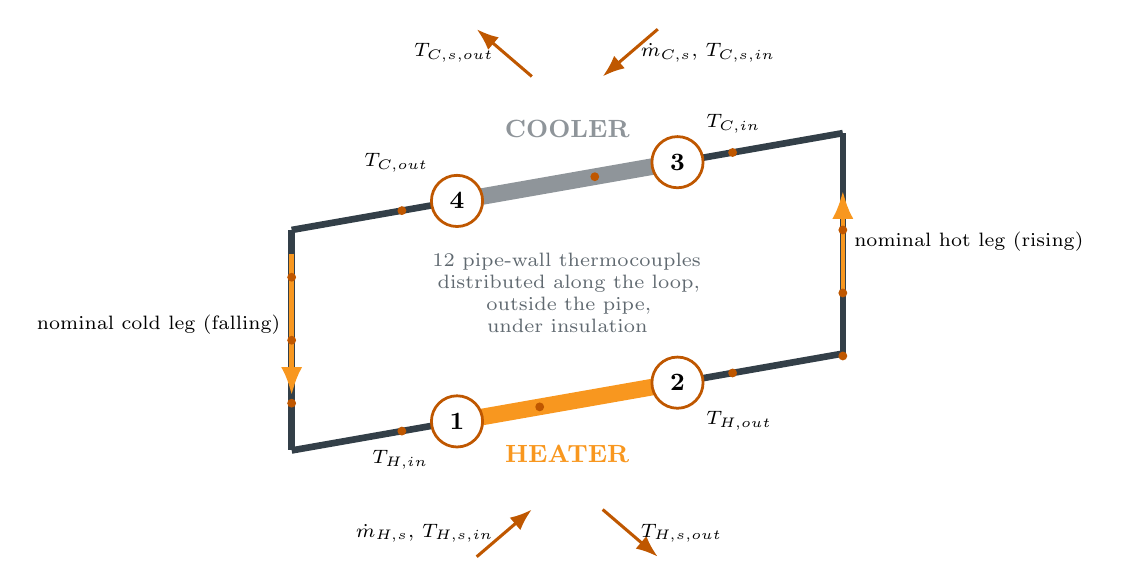
\begin{tikzpicture}[
  x=1cm,y=1cm,
  pipe/.style={line width=2.4pt,draw=Navy},
  heat/.style={line width=6pt,draw=Warn},
  cool/.style={line width=6pt,draw=Navy!55!white},
  sensor/.style={circle,draw=Teal,fill=white,line width=1pt,minimum size=6.5mm,font=\small\bfseries},
  secondary/.style={-Latex,draw=Teal,line width=1.1pt},
  flow/.style={-Latex,draw=Warn,line width=1.6pt}
]
  % corner coordinates: vertical legs at x=0 (cold) and x=7 (hot); heater/cooler diagonals at ~10 deg
  \coordinate (BL) at (0,0.6);
  \coordinate (BR) at (7,1.83);
  \coordinate (TR) at (7,4.63);
  \coordinate (TL) at (0,3.4);


  \coordinate (TOne)   at ($(BL)!0.30!(BR)$); % heater inlet
  \coordinate (TTwo)   at ($(BL)!0.70!(BR)$); % heater outlet
  \coordinate (TThree) at ($(TR)!0.30!(TL)$); % cooler inlet
  \coordinate (TFour)  at ($(TR)!0.70!(TL)$); % cooler outlet

  % pipe legs
  \draw[pipe] (TL) -- (BL); % cold leg (left, vertical)
  \draw[pipe] (BR) -- (TR); % hot leg  (right, vertical)
  % heater (lower diagonal) and cooler (upper diagonal)
  \draw[pipe] (BL) -- (BR);
  \draw[pipe] (TR) -- (TL);
  \draw[heat] (TOne) -- (TTwo);
  \draw[cool] (TThree) -- (TFour);
  \node[font=\small\bfseries,text=Warn] at (3.5,0.55) {HEATER};
  \node[font=\small\bfseries,text=Navy!55!white] at (3.5,4.68) {COOLER};

  % station sensors at the active-section boundaries
  \node[sensor,label=below left:{\scriptsize $T_{H,in}$}] at (TOne) {1};
  \node[sensor,label=below right:{\scriptsize $T_{H,out}$}] at (TTwo) {2};
  \node[sensor,label=above right:{\scriptsize $T_{C,in}$}] at (TThree) {3};
  \node[sensor,label=above left:{\scriptsize $T_{C,out}$}] at (TFour) {4};

  % flow direction: up the hot leg, down the cold leg
  \draw[flow] (7,2.6) -- (7,3.9) node[midway,right,font=\scriptsize] {nominal hot leg (rising)};
  \draw[flow] (0,3.1) -- (0,1.3) node[midway,left,font=\scriptsize] {nominal cold leg (falling)};

  % heater secondary (below) and cooler secondary (above)
  \draw[secondary] (2.35,-0.75) -- (3.05,-0.15) node[midway,left,font=\scriptsize] {$\dot m_{H,s},\,T_{H,s,in}$};
  \draw[secondary] (3.95,-0.15) -- (4.65,-0.75) node[midway,right,font=\scriptsize] {$T_{H,s,out}$};
  \draw[secondary] (3.05,5.35) -- (2.35,5.95) node[midway,left,font=\scriptsize] {$T_{C,s,out}$};
  \draw[secondary] (4.65,5.95) -- (3.95,5.35) node[midway,right,font=\scriptsize] {$\dot m_{C,s},\,T_{C,s,in}$};

  % 12 wall thermocouples distributed along legs
  \foreach \yy in {1.2,2.0,2.8} {
    \fill[Teal] (0,\yy) circle (1.6pt);
    \fill[Teal] (7,\yy+0.6) circle (1.6pt);
  }
  \foreach \tt in {0.2,0.45,0.8} {
    \fill[Teal] ($(BL)!\tt!(BR)$) circle (1.6pt);
    \fill[Teal] ($(TR)!\tt!(TL)$) circle (1.6pt);
  }
  \node[font=\scriptsize,align=center,text=MidGray,text width=3.8cm] at (3.5,2.6)
    {12 pipe-wall thermocouples\\ distributed along the loop,\\ outside the pipe, under insulation};
\end{tikzpicture}
\caption{STNCL schematic, not to scale.}
\label{fig:schematic}
\end{figure}

% -----------------------------------------------------------------------------
\subsection{Definitions and Conventions}

\subsubsection{Primary fluid temperatures}
\label{sec:def_temps}

Using the station numbering of Figure~\ref{fig:schematic} ($T_{H,in}$: heater inlet, $T_{H,out}$: heater outlet, $T_{C,in}$: cooler inlet, $T_{C,out}$: cooler outlet), the nominal hot-leg, cold-leg, and four-point mean temperatures are
\begin{align}
\Thot &= \frac{T_{H,out}+T_{C,in}}{2}, \\
\Tcold &= \frac{T_{C,out}+T_{H,in}}{2}, \\
\Tavg &= \frac{T_{H,in}+T_{H,out}+T_{C,in}+T_{C,out}}{4}, \\
\Delta T_{\mathrm{loop}} &= \Thot-\Tcold.
\end{align}

The exchanger temperature changes are
\begin{align}
\Delta T_H &= T_{H,out}-T_{H,in}, \\
\Delta T_C &= T_{C,in}-T_{C,out},
\end{align}
where the signs assume the nominal circulation direction shown in Figure~\ref{fig:schematic}. For the documented primary-fluid composition $c$, define the corresponding primary enthalpy changes as
\begin{align}
\Delta h_H &= h(T_{H,out},c)-h(T_{H,in},c), \\
\Delta h_C &= h(T_{C,in},c)-h(T_{C,out},c).
\end{align}
These differences retain the same sign convention and are evaluated from the approved property source.

\subsubsection{Secondary-side thermal duties}
\label{sec:secondary_duty}

Define positive heater duty as heat supplied by the heater secondary circuit and positive cooler duty as heat removed by the cooler secondary circuit:
\begin{align}
\QHs &= \dot m_{H,s}\left(h_{H,s,in}-h_{H,s,out}\right), \\
\QCs &= \dot m_{C,s}\left(h_{C,s,out}-h_{C,s,in}\right).
\end{align}

The actual signs shall be verified from the measured secondary flow directions. Enthalpy differences are preferred to a constant-$c_p$ approximation. A single documented property reference (source, composition or concentration, pressure convention, and version) shall be fixed for each fluid and used consistently for every enthalpy $h(T,c)$, density $\rho(T,c)$, and viscosity $\mu(T,c)$ evaluation throughout the reduction, including the flow-inference and Reynolds-number relations defined in \PhaseFourDoc, Section~``Primary-flow and Reynolds-number inference. 

\subsubsection{Ambient heat-transfer sign convention}

For any primary-loop region $j$, define $\dot Q_{a,j}>0$ when heat leaves the loop and enters the room. A below-ambient region that gains heat from the room therefore has $\dot Q_{a,j}<0$.

At whole-loop steady state,
\begin{equation}
\dot Q_{a,\mathrm{total}}=\QHs-\QCs.
\label{eq:whole_loop_loss}
\end{equation}

Equation~\eqref{eq:whole_loop_loss} is the primary integral measurement of whole-loop heat loss or gain. It is valid when thermal storage is negligible and the secondary measurement planes adequately bound the heater and cooler.


% -----------------------------------------------------------------------------


\clearpage
\section{Procedure}
\label{sec:procedure}
\label{sec:test_procedure}
\label{sec:phase0}
\subsection{Campaign execution conventions}
Unless otherwise stated, the automated data-acquisition system shall record all available measurement, environmental, control-state, alarm, interlock, and event channels continuously throughout each test. Operator records shall identify manual actions, configuration changes, unusual observations, and the accepted analysis interval. These recording and configuration-control requirements apply to Phases~1--4 by reference.

Each phase shall receive one of three dispositions:
\begin{description}
    \item[Proceed.] The phase objectives were met and the data are suitable for their intended use. Any limitations shall be documented.
    \item[Repeat.] One or more required activities or runs did not provide complete or usable data.
    \item[Additional work required.] The data are valid, but a targeted test, measurement correction, procedure change, or model revision is required before the next dependent phase.
\end{description}

\subsection{Method}

Complete the following activities before beginning Phase~1:

\begin{enumerate}
    \item \textbf{Document the facility and fluid configuration.}
    \begin{enumerate}
        \item Record valve and bypass positions, expansion-tank condition, insulation condition, temporary instrumentation, and primary-fluid inventory.
        \item Record the Prop-30 concentration, batch, selected property correlation, and available contamination or water-content information.
        \item Assign a unique configuration identifier for use in all test and analysis records.
    \end{enumerate}

    \item \textbf{Verify the geometry and model map.}
    \begin{enumerate}
        \item Record pipe dimensions and material, insulation type and thickness, fittings, supports, heater and cooler boundaries, and wall-thermocouple locations.
        \item Confirm that each measurement location can be mapped to the corresponding system-code cell or CFD region.
    \end{enumerate}

    \item \textbf{Verify instrumentation documentation.}
    \begin{enumerate}
        \item Confirm the physical location and installed coupling of every thermocouple and Luna measurement.
        \item Archive available calibration, correction, residual, range, sampling-rate, and uncertainty information.
        \item Confirm that each reported channel contains the intended calibrated quantity.
        \item Approve an acceptance-channel matrix that designates, for each acceptance class and intended use, every signal as mandatory, an approved alternate, or diagnostic only. A Luna channel may substitute for an internal thermocouple only when Phase~1 demonstrates adequate agreement and the substitution is approved before the affected run is evaluated.
    \end{enumerate}

    \item \textbf{Document the secondary-side energy-balance boundaries.}
    \begin{enumerate}
        \item Identify the heater- and cooler-side inlet and outlet temperature locations and flow directions.
        \item Record flow-meter calibration information and the applicable secondary-fluid property correlations.
        \item Identify unmeasured piping or heat transfer between each measurement boundary and its heat exchanger.
    \end{enumerate}

    \item \textbf{Verify environmental and condensation measurements.}
    \begin{enumerate}
        \item Confirm two synchronized room-temperature and relative-humidity stations, one near the nominal hot leg and one near the nominal cold leg.
        \item Confirm surface-temperature measurements near the coldest expected exposed locations.
        \item Establish the condensation-classification procedure using
        \begin{equation}
            \Delta T_{\mathrm{dew}}
            =
            T_{\mathrm{surface,min}}-T_{\mathrm{dew}}.
        \end{equation}
        Classify a condition as dry when $\Delta T_{\mathrm{dew}}\geq\SI{3}{\degreeCelsius}$, near dew point when $0\leq\Delta T_{\mathrm{dew}}<\SI{3}{\degreeCelsius}$, condensing when $\Delta T_{\mathrm{dew}}<0$ or visible condensation is present, and unknown when the coldest exposed surface is not instrumented. Visible condensation overrides the calculated classification.
    \end{enumerate}

    \item \textbf{Verify logging and time synchronization.}
    \begin{enumerate}
        \item Confirm recording of heater and cooler commands, setpoints, states, controller outputs, secondary flow rates, valve positions, alarms, interlocks, and operator events.
        \item Establish a common clock or document the offset of each acquisition system.
        \item Introduce a common event or signal change and verify consistent timing across the recorded data streams.
    \end{enumerate}

    \item \textbf{Document approved operating limits.}
    Record the approved limits for primary-fluid, component, surface, and room temperatures; pressure; heater and cooler duty; secondary-side flow; expansion-tank level; and fill and drain operations.

    \item \textbf{Perform the coordinated acquisition checkout.}
    \begin{enumerate}
        \item Initialize the acquisition and control systems and begin synchronized recording.
        \item Verify that every required channel is present, plausible, and time aligned.
        \item Archive a short checkout record demonstrating readiness for Phase~1.
    \end{enumerate}
\end{enumerate}

\subsection{Phase 0 Run ID}
None.

\subsection{Analysis and Required Outputs}

Confirm that the Phase~0 records are complete and internally consistent. Resolve missing channel mappings, calibration information, time offsets, operating limits, or configuration details before quantitative testing. The required output is an approved readiness record containing the configuration identifier, channel and geometry maps, the acceptance-channel matrix and any approved alternates, measurement uncertainties, synchronization verification, operating limits, condensation-classification method, and checkout data set.

\subsection{Disposition}

Assign \textbf{Proceed} when the readiness record supports the planned measurements and analyses. Assign \textbf{Repeat} when the checkout data are incomplete or unusable. Assign \textbf{Additional work required} when instrumentation, documentation, synchronization, or facility configuration must be corrected before Phase~1.

No experimental test phase shall begin until Phase~0 is dispositioned as \textbf{Proceed}.

% -----------------------------------------------------------------------------

\clearpage
\appendix
\section{Nomenclature}
\label{sec:nomenclature}
A dot denotes a rate, a hat denotes an estimate or model prediction, an overbar denotes an interval or block mean as stated in context, and $u_x$ denotes the standard uncertainty of quantity $x$. Only symbols used in this phase document are included below.

\begingroup
\footnotesize
\setlength{\LTpre}{4pt}
\setlength{\LTpost}{10pt}
\setlength{\tabcolsep}{4pt}
\renewcommand{\arraystretch}{1.10}
\begin{longtable}{@{}>{\raggedright\arraybackslash}p{1.78in}>{\raggedright\arraybackslash}p{1.08in}>{\raggedright\arraybackslash}p{3.62in}@{}}
\caption{Phase 0 nomenclature.}\label{tab:nomenclature}\\
\toprule
\textbf{Symbol} & \textbf{Units} & \textbf{Description} \\
\midrule
\endfirsthead
\multicolumn{3}{l}{\small\itshape Table~\ref{tab:nomenclature} continued from previous page}\\
\toprule
\textbf{Symbol} & \textbf{Units} & \textbf{Description} \\
\midrule
\endhead
\bottomrule
\endfoot
$T$ & \si{\degreeCelsius} & Generic measured temperature. \\
$T_{H,in},T_{H,out},T_{C,in},T_{C,out}$ & \si{\degreeCelsius} & Primary temperatures at the heater and cooler measurement planes. \\
$T_{H,s,in/out},T_{C,s,in/out}$ & \si{\degreeCelsius} & Secondary inlet and outlet temperatures at the heater and cooler boundaries. \\
$T_j,\,T_{w,i}$ & \si{\degreeCelsius} & Generic internal-fluid and under-insulation wall temperatures. \\
$\Tamb,\,T_{\mathrm{amb},i}$ & \si{\degreeCelsius} & Representative and region-specific room-air temperatures. \\
$T_{\mathrm{surface,min}},\,T_{\mathrm{dew}},\,\Delta T_{\mathrm{dew}}$ & \si{\degreeCelsius} & Minimum exposed-surface temperature, dew point, and exposed-surface margin above dew point. \\
$\Thot,\,\Tcold,\,\Tavg,\,\Delta T_{\mathrm{loop}}$ & \si{\degreeCelsius} & Hot-leg, cold-leg, four-point mean, and loop temperature-difference coordinates. \\
$\Delta T_H,\,\Delta T_C$ & \si{\degreeCelsius} & Signed primary temperature changes across the heater and cooler. \\
$\QHs,\,\QCs$ & \si{\watt} & Heater duty supplied and cooler duty removed on the secondary side. \\
$\dot Q_{a,j},\,\dot Q_{a,\mathrm{total}}$ & \si{\watt} & Regional and whole-loop ambient heat exchange; positive to the room. \\
$h(T,c),\,\Delta h_H,\,\Delta h_C$ & \si{\joule\per\kilogram} & Specific enthalpy and signed primary exchanger enthalpy changes. \\
$c_p(T,c),\,\rho(T,c),\,\mu(T,c)$ & Mixed & Heat capacity, density, and dynamic viscosity for documented composition $c$. \\
$\dot m_{H,s},\,\dot m_{C,s}$ & \si{\kilogram\per\second} & Heater and cooler secondary mass-flow rates. \\
$i,j,k,m,\ell,\mathcal N_i,c$ & -- & Measurement/model indices, coupled-region set, and documented fluid composition. \\
\end{longtable}
\endgroup

\end{document}
